\section{ПРАКТИЧЕСКАЯ ЧАСТЬ}
\subsection{Алгоритм работы}

В приложения ONMP врач прикрепляет сделанную им ранее фотографию ЭКГ.
Изображено на рисунке~\ref{fig:fig1}.
\begin{figure}
  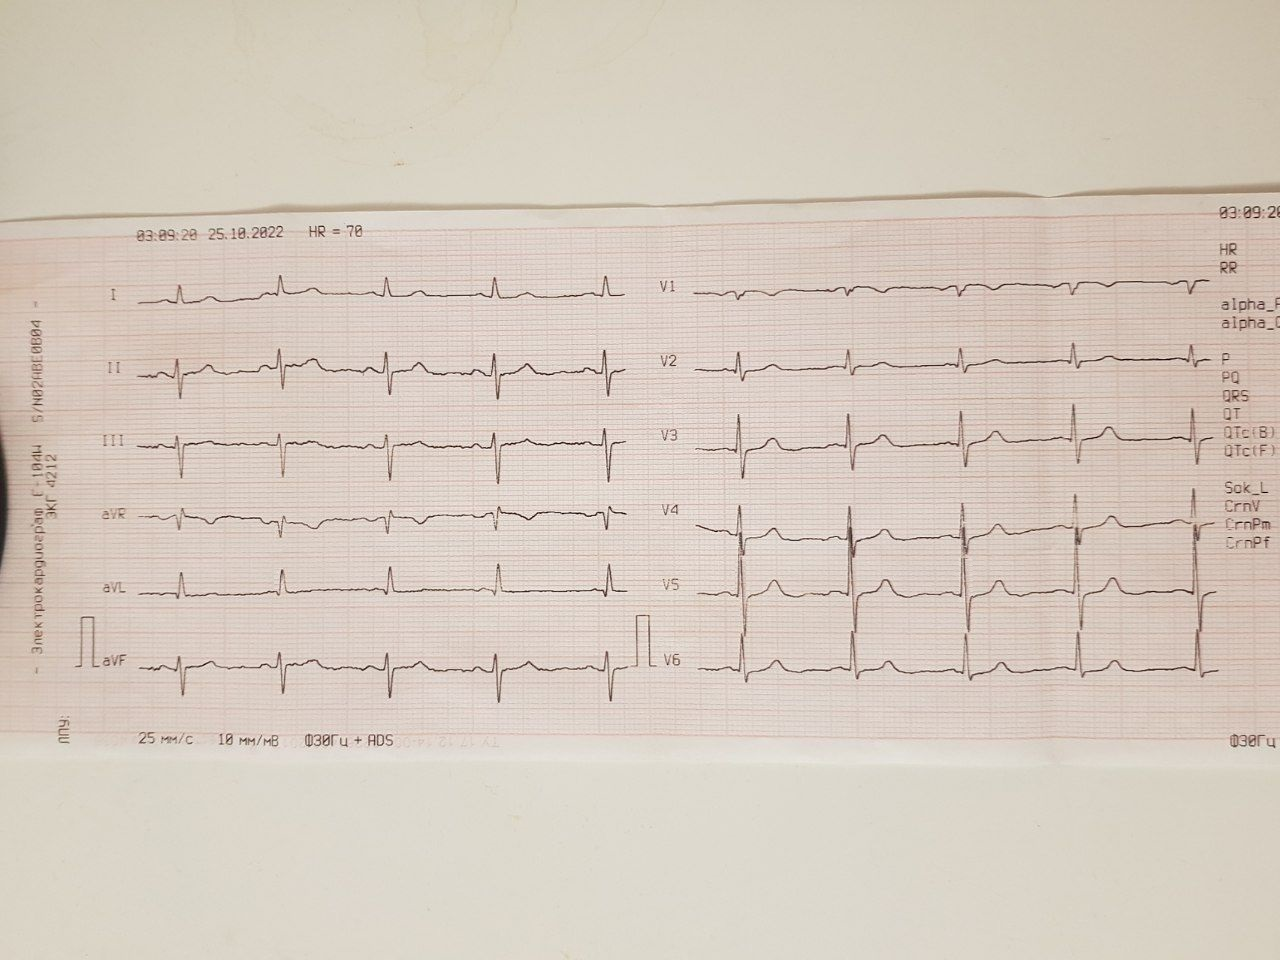
\includegraphics[scale=0.45]{inc/1}
  \caption{Оригинальная фотография ЭКГ.}
  \label{fig:fig1}
\end{figure}

Изменение размера и выранивание изображения, полезно для стандартизации размеров и соотношения сторон графика. Изображено на рисунке~\ref{fig:fig2}. Это также дополнительно может помочь снизить вычислительную нагрузку и упростить последующие этапы обработки.

\begin{figure}
  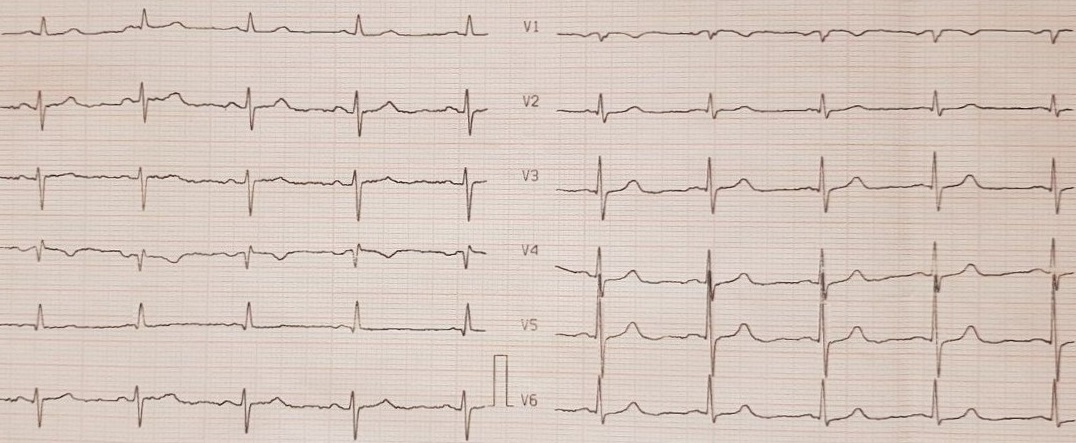
\includegraphics[scale=0.5]{inc/2}
  \caption{Выравнивание, стандартизация и обрезание.}
  \label{fig:fig2}
\end{figure}

Если рассматривать каждый график отведений ЭКГ отдельно, это упрощает задачу обнаружения и оцифровки графика. Изображено на рисунке~\ref{fig:fig3}. Сосредоточившись на одном графике за один раз, процесс становится более упорядоченным.

Было принято решение отказаться от бинаризации, которая предполагает преобразование графика ЭКГ в двоичный формат изображения. Хотя бинаризация обычно используется для сегментации изображений и повышения контрастности, иногда она может привести к потере важной информации или усложнить определение контуров, особенно в случае с графиками ЭКГ.

\begin{figure}
  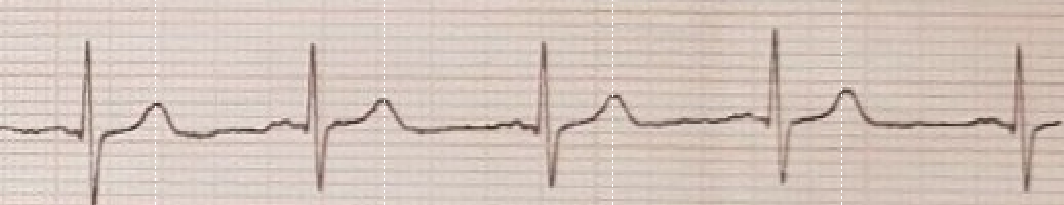
\includegraphics[scale=0.5]{inc/3}
  \caption{Выделение каждого ответвления ЭКГ.}
  \label{fig:fig3}
\end{figure}

Преобразуя изображение ЭКГ в градации серого на рисунке~\ref{fig:fig4}, мы упрощаем последующие задачи обработки и анализа изображения. Изображения в градациях серого содержат только один канал информации, представляющий интенсивность или яркость каждого пикселя. 

\begin{figure}
  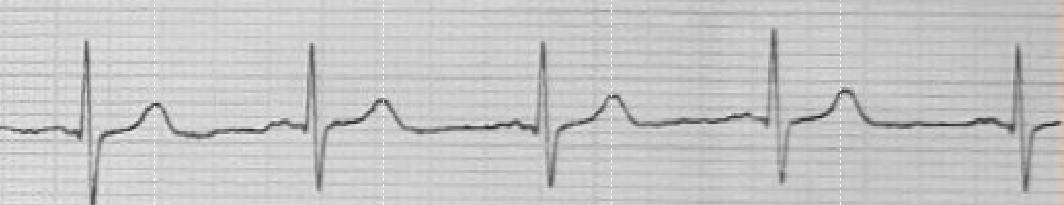
\includegraphics[scale=0.5]{inc/4}
  \caption{Градации серого.}
  \label{fig:fig4}
\end{figure}

Преобразование изображения в его негатив на рисунке~\ref{fig:fig5} - это распространенная операция обработки изображений, которая заключается в инвертировании значений градаций серого цвета изображения. Эта операция также известна как отрицание изображения или инверсия изображения.

Цель преобразования изображения в негатив - повысить контрастность и выявить детали в форме волны ЭКГ. При инвертировании значений шкалы серого темные области становятся светлее, а светлые - темнее, что приводит к изменению общего тона изображения.

\begin{figure}
  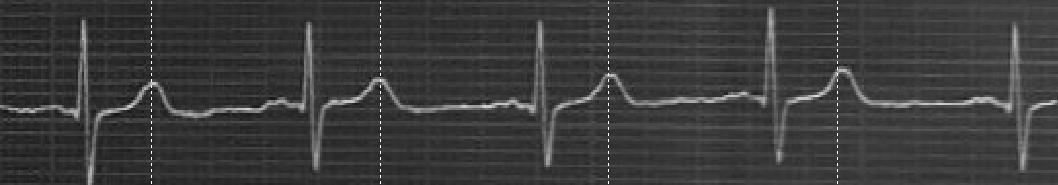
\includegraphics[scale=0.5]{inc/5}
  \caption{Негатив.}
  \label{fig:fig5}
\end{figure}

Регулировка контрастности изображения является важнейшим этапом анализа ЭКГ для улучшения видимости графика и удаления нежелательной сетки или фонового шума. Регулировка контрастности включает в себя изменение диапазона значений градаций серого в изображении, тем самым увеличивая различие между различными интенсивностями.

Изменяя контрастность изображения, мы можем подчеркнуть график ЭКГ изображено на рисунке~\ref{fig:fig6} и одновременно минимизировать влияние сетки или фона. Такая настройка помогает лучше визуализировать и анализировать особенности и характеристики формы волны.

\begin{figure}
  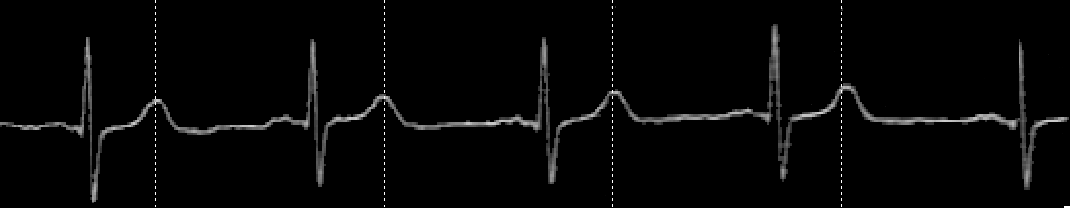
\includegraphics[scale=0.5]{inc/6}
  \caption{Контрастность.}
  \label{fig:fig6}
\end{figure}

Выделение контура графика ЭКГ на рисунке~\ref{fig:fig7}, который в дальнейшем будет оцифрован.

\begin{figure}
  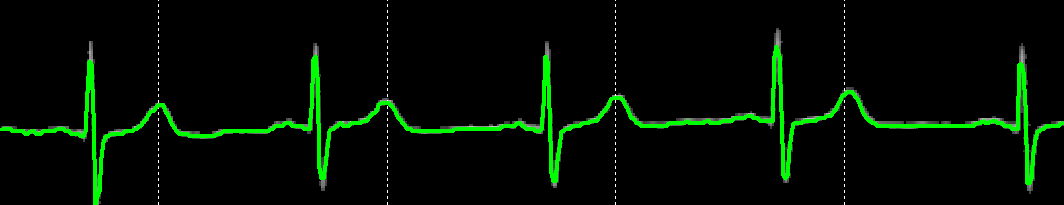
\includegraphics[scale=0.5]{inc/7}
  \caption{Выделение контура.}
  \label{fig:fig7}
\end{figure}

Демонстрация самого контура графика ЭКГ на рисунке~\ref{fig:fig8}.

\begin{figure}
  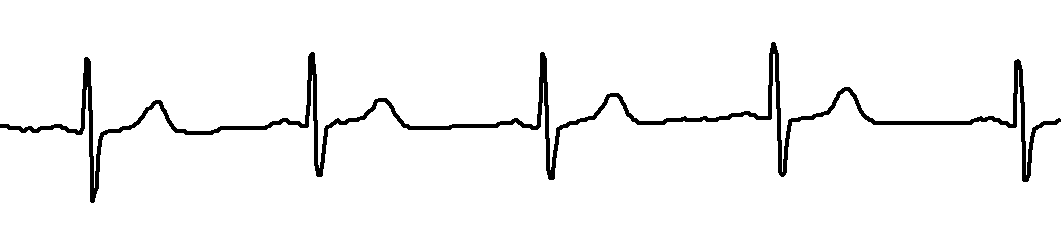
\includegraphics[scale=0.5]{inc/0}
  \caption{Контур.}
  \label{fig:fig8}
\end{figure}

Наложение полученного контура на оригинальную картинку, которая на рисунке~\ref{fig:fig9}. 

\begin{figure}
  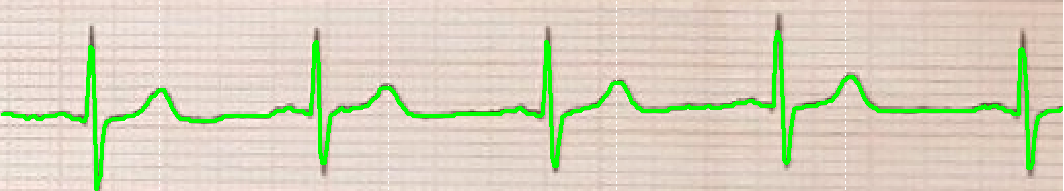
\includegraphics[scale=0.5]{inc/00}
  \caption{Контур и изначальная картинка.}
  \label{fig:fig9}
\end{figure}

Затем происходит оцифровка отведения ЭКГ в файл для анализа, оцифровка отображена на рисунке~\ref{fig:fig10}.

\begin{figure}
  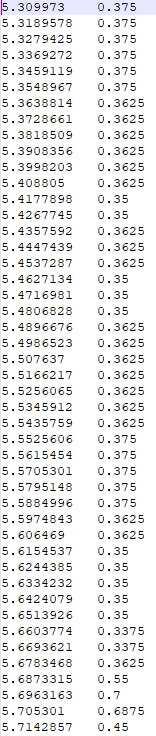
\includegraphics[scale=1.1]{inc/8}
  \caption{Оцифровка отведения ЭКГ.}
  \label{fig:fig10}
\end{figure}

Далее каждое отведение сохраняется и анализируется.

Применяется алгоритмы извлечения характеристик ЭКГ, таких как Р-волны, комплексы QRS, Т-волны, ритм, регулярность, ЧЖС, ЭОС.

Далее рассчитываются соответствующие показатели, такие как частота сердечных сокращений, интервал PR, интервал QT и измерения сегмента ST.
Сравнивается с нормальными диапазонами.


Вывод результатов:
Отображение извлеченных характеристик ЭКГ, показателей и результатов анализа в виде отчета отображенного на рисунке~\ref{fig:fig11}.


\begin{figure}
  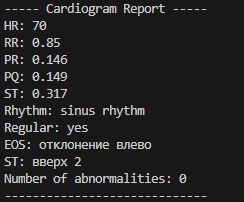
\includegraphics[scale=1.1]{inc/0000}
  \caption{Вывод результата}
  \label{fig:fig11}
\end{figure}

\subsection{Тестирование}

Точность оцифровки ЭКГ:
Оцифровка ЭКГ включает преобразование аналогового сигнала ЭКГ в цифровой формат, что позволяет эффективно хранить, анализировать и передавать сигнал. Точность оцифровки ЭКГ является решающим фактором в обеспечении надежных результатов диагностики. В данном исследовании был проведен комплексный процесс оцифровки. Точность оцифровки оценивалась на основе сравнения оригинальной аналоговой ЭКГ и оцифрованной версии.

Результаты показали, что в процессе оцифровки ЭКГ была достигнута впечатляющая точность 0,97. Такой высокий уровень точности указывает на точность, с которой цифровое представление отражает основные особенности и характеристики оригинальной аналоговой ЭКГ. Точная оцифровка обеспечивает прочную основу для последующего анализа и интерпретации, способствуя повышению точности диагностики.

Точность определения базовой линии ЭКГ:
Базовая линия ЭКГ представляет собой электрическую активность сердца, когда оно находится в состоянии покоя. Определение базовой линии является важным этапом предварительной обработки при анализе ЭКГ, поскольку оно устраняет блуждание базовой линии, облегчая точную оценку других характеристик ЭКГ. В данном исследовании были реализованы различные методы определения базовой линии, которые оценивались на предмет их точности.

Результаты показали, что точность обнаружения базовой линии ЭКГ составляет 0,87. Хотя такой уровень точности указывает на надежное удаление базовой линии, важно учитывать ограничения и проблемы, связанные с обнаружением базовой линии. Такие факторы, как шумовые помехи, различные характеристики базовой линии у разных людей и артефакты, могут повлиять на точность определения базовой линии. Поэтому для повышения точности алгоритмов обнаружения базовой линии необходимы дальнейшие исследования и усовершенствования.

Последствия и будущие направления:
Высокая точность, достигнутая при оцифровке ЭКГ (0,97), подчеркивает эффективность использованных методов в точном представлении аналогового сигнала ЭКГ в цифровой форме. Такая точность позволяет врачам и исследователям уверенно анализировать и интерпретировать цифровые данные ЭКГ, что приводит к более точным диагнозам и решениям о лечении.



